% =============================================================================
%  Section 4.3 — Triển khai và kiểm nghiệm với người dùng
%  Subsections:
%    4.3.1  Triển khai và vận hành
%    4.3.2  Giao diện người dùng
%    4.3.3  Thiết kế kiểm nghiệm với người dùng
%    4.3.4  Kết quả kiểm nghiệm với người dùng
%    4.3.5  Thảo luận trải nghiệm thực tế
% =============================================================================

\section{Triển khai và kiểm nghiệm với người dùng}
\label{sec:user_deployment}

Song song với các thí nghiệm định lượng ở Mục~\ref{sec:experiments}, hệ thống được triển khai lên hạ tầng đám mây và đưa vào kiểm nghiệm qua hai hình thức thực nghiệm: chấm điểm đa tiêu chí và đánh giá so sánh.

\subsection{Triển khai và vận hành}

Hệ thống được triển khai dưới dạng ứng dụng web đám mây. Người dùng truy cập thông qua trình duyệt trên máy tính hoặc điện thoại mà không cần cài đặt phần mềm; máy chủ được đặt tại khu vực Đông Nam Á để đảm bảo độ trễ thấp cho người dùng tại Việt Nam. Cơ chế tự động mở rộng tài nguyên theo lưu lượng truy cập giúp hệ thống đáp ứng ổn định khi nhiều người tham gia khảo sát đồng thời.

Hệ thống vận hành theo hai chế độ tương ứng với hai hình thức kiểm nghiệm (Mục~\ref{sec:user_study}). Ở chế độ trực tiếp, ba pipeline GraphRAG, RAG truyền thống và LLM-only chạy đồng thời ngay khi người dùng đặt câu hỏi và trả kết quả trong vài chục giây. Ở chế độ so sánh, câu trả lời của ba hệ thống cho các câu hỏi chuẩn bị sẵn đã được sinh trước và lưu trữ; người dùng chỉ đọc kết quả đã cache, vừa giảm thời gian chờ, vừa đảm bảo mọi người tham gia đánh giá trên cùng một tập câu trả lời.

\subsection{Giao diện người dùng}

Giao diện là ứng dụng web đa trang. Hai trang chính phục vụ kiểm nghiệm được đặt tên tương ứng hai hình thức: trang \textbf{Experiment} cho phép người dùng tự đặt câu hỏi và đánh giá trực tiếp; trang \textbf{Preference} hiển thị câu trả lời đã chuẩn bị sẵn để người dùng chọn phương án tốt nhất. Giao diện tổng quan được trình bày ở Hình~\ref{fig:UI}.

\begin{figure}[!ht]
    \centering
    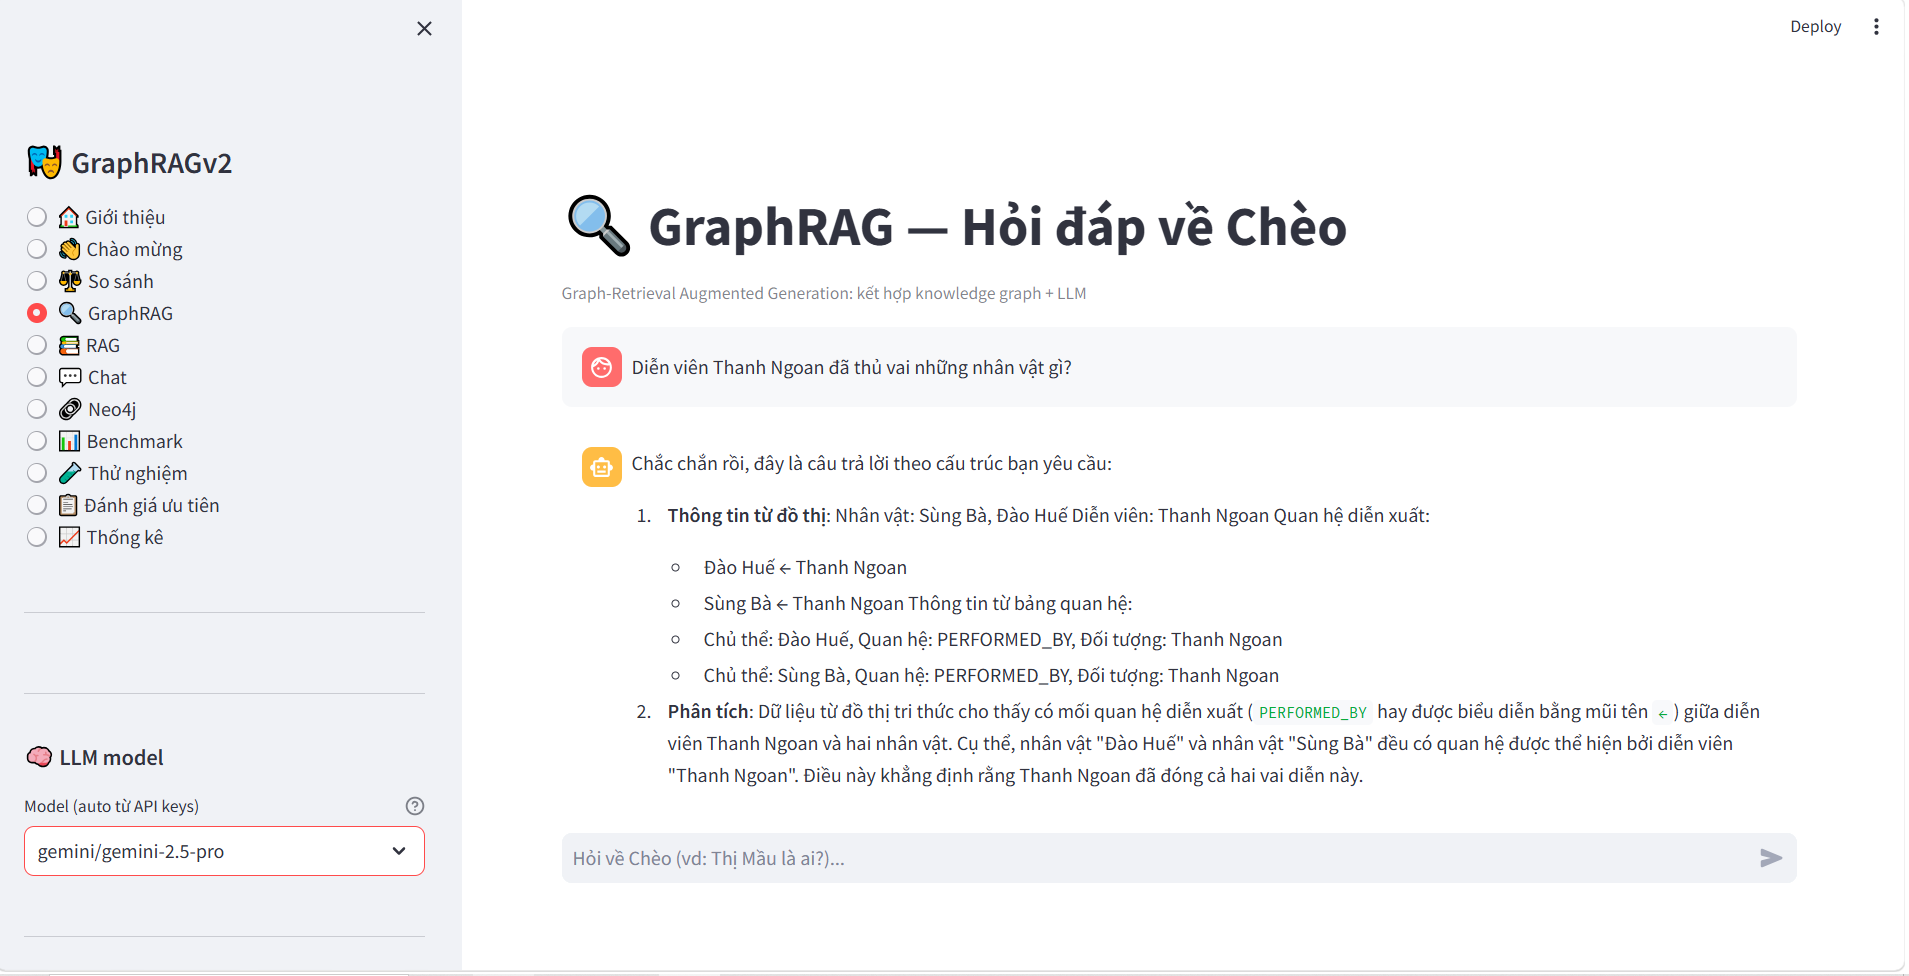
\includegraphics[width=1\linewidth]{figures//c4/UI.png}
    \caption{Giao diện thử nghiệm của hệ thống.}
    \label{fig:UI}
\end{figure}

\subsection{Thiết kế kiểm nghiệm với người dùng}
\label{sec:user_study}

\subsubsection{Chấm điểm đa tiêu chí}
\label{sec:experiment_study}

Hình thức thực nghiệm đầu tiên sử dụng trang Experiment (\textbf{Hình \ref{fig:experiment}}), cho phép người tham gia tự đặt câu hỏi và chấm điểm câu trả lời của ba hệ thống trong thời gian thực. Thử nghiệm tổ chức theo bốn bước: ba bước đầu yêu cầu chọn một câu hỏi trong số bảy câu chuẩn bị sẵn tại mỗi mức độ Dễ, Trung bình và Khó; bước cuối cho phép đặt một câu hỏi tự do. Thiết kế này vừa đảm bảo có câu hỏi có ground truth để so sánh giữa các người tham gia, vừa khảo sát được các câu hỏi tự phát phản ánh nhu cầu thực.

\begin{figure}
    \centering
    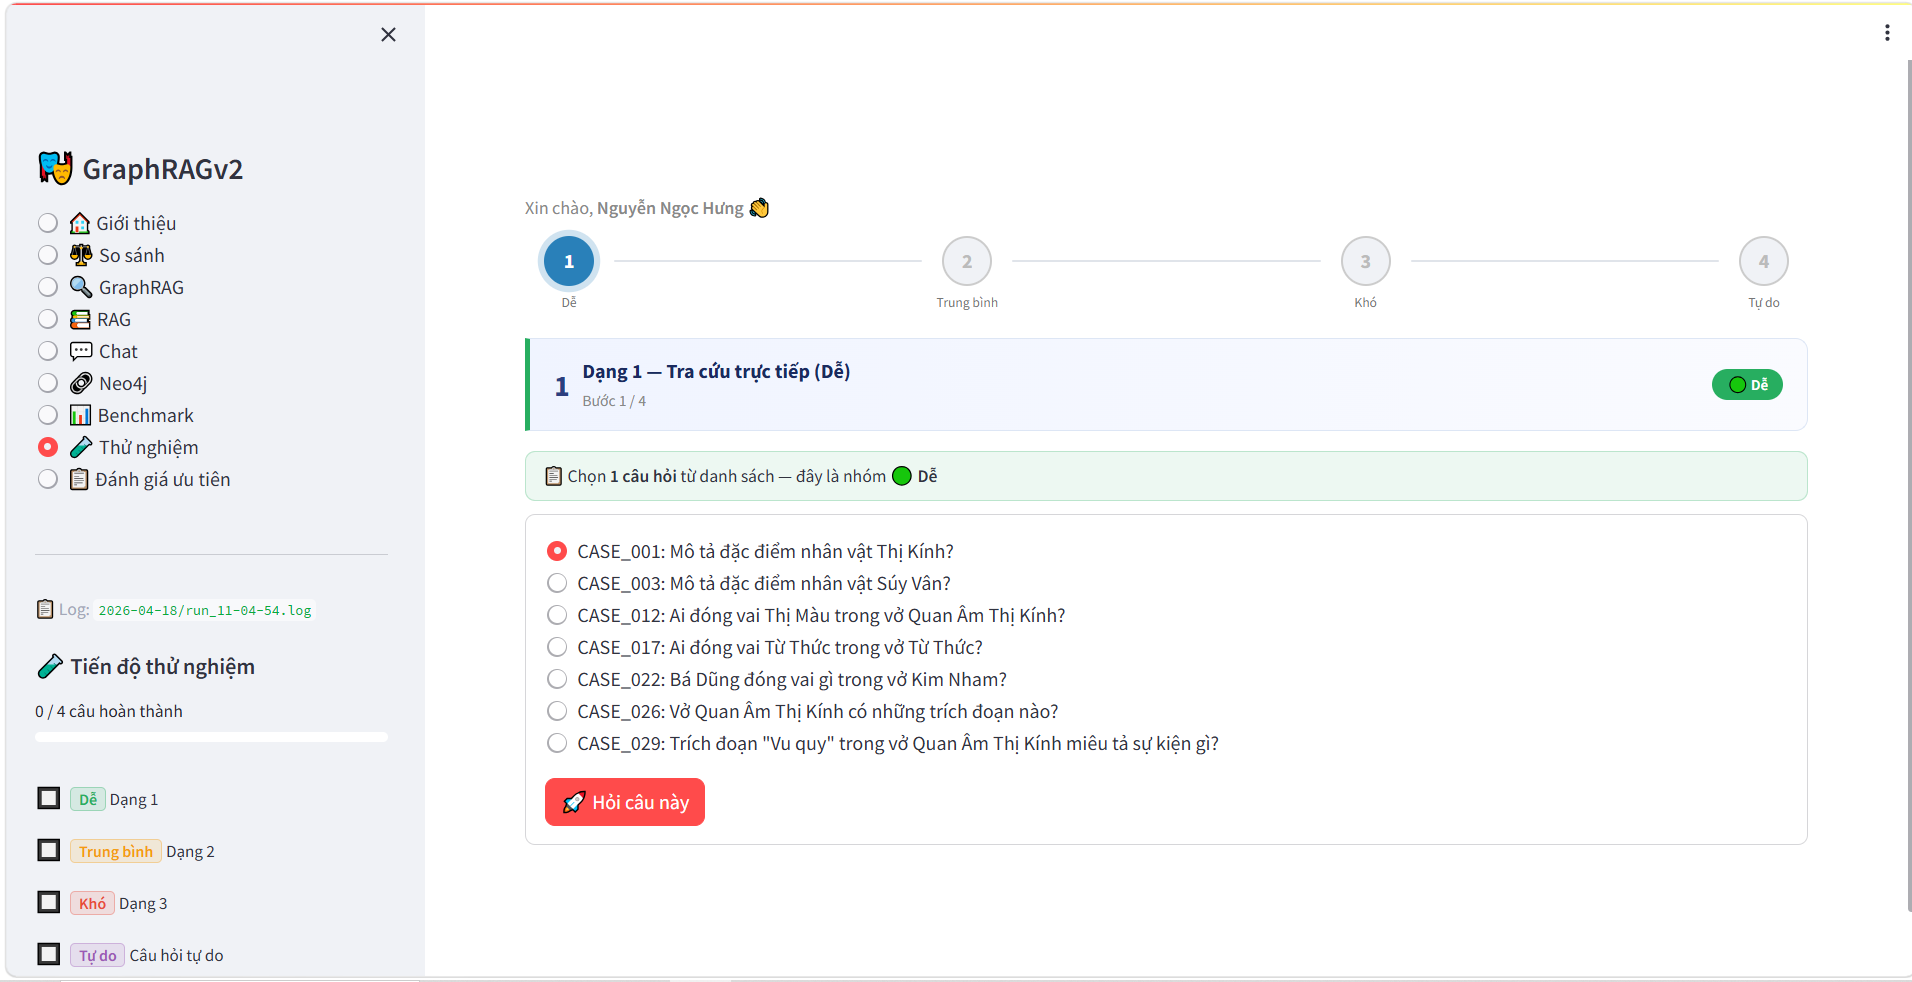
\includegraphics[width=0.9\linewidth]{figures//c4/Experiment.png}
    \caption{Giao diện thực nghiệm hỏi đáp}
    \label{fig:experiment}
\end{figure}

Với mỗi câu, hệ thống chạy đồng thời ba pipeline và hiển thị câu trả lời song song trong ba cột ẩn danh. Người tham gia chấm điểm từng hệ thống theo ba tiêu chí trên thang 1--5: \textit{Chính xác} (thông tin có đúng không), \textit{Đầy đủ} (bao quát nội dung câu hỏi) và \textit{Tự nhiên} (dễ đọc, mạch lạc); đồng thời chọn hệ thống tổng thể tốt nhất. Sau bốn bước, người tham gia trả lời khảo sát hậu nghiệm về mức độ hiểu biết Chèo, tần suất sử dụng công cụ AI, tiêu chí đặt nặng nhất khi lựa chọn và các loại lỗi thường gặp.

Đối tượng tham gia hình thức này là sinh viên, đại diện cho người dùng phổ thông không có kiến thức chuyên sâu về Chèo. Cách chọn đối tượng này nhằm phản ánh trải nghiệm cảm nhận của đông đảo người dùng cuối trong bối cảnh không có điều kiện thẩm định từng chi tiết tri thức. Thông tin hậu nghiệm cho phép phân tích kết quả theo các phân nhóm --- chẳng hạn nhóm có hiểu biết Chèo so với nhóm không có, hoặc nhóm sử dụng AI thường xuyên so với nhóm ít sử dụng.

\subsubsection{Đánh giá so sánh}
\label{sec:preference_study}

Hình thức thực nghiệm thứ hai sử dụng trang Preference (\textbf{Hình \ref{fig:preference}}). Hai mươi mốt câu hỏi tiêu biểu được chọn từ CheoBench v2, bao phủ cả ba nhóm độ khó và nhiều dạng truy vấn từ tra cứu trực tiếp đến phân tích liên vở. Câu trả lời của ba hệ thống đã được sinh sẵn và lưu trữ; người tham gia đọc đồng thời ba câu trả lời hiển thị ẩn danh trong ba cột, chọn câu trả lời tốt nhất và có thể ghi chú nhận xét cho từng câu.

\begin{figure}
    \centering
    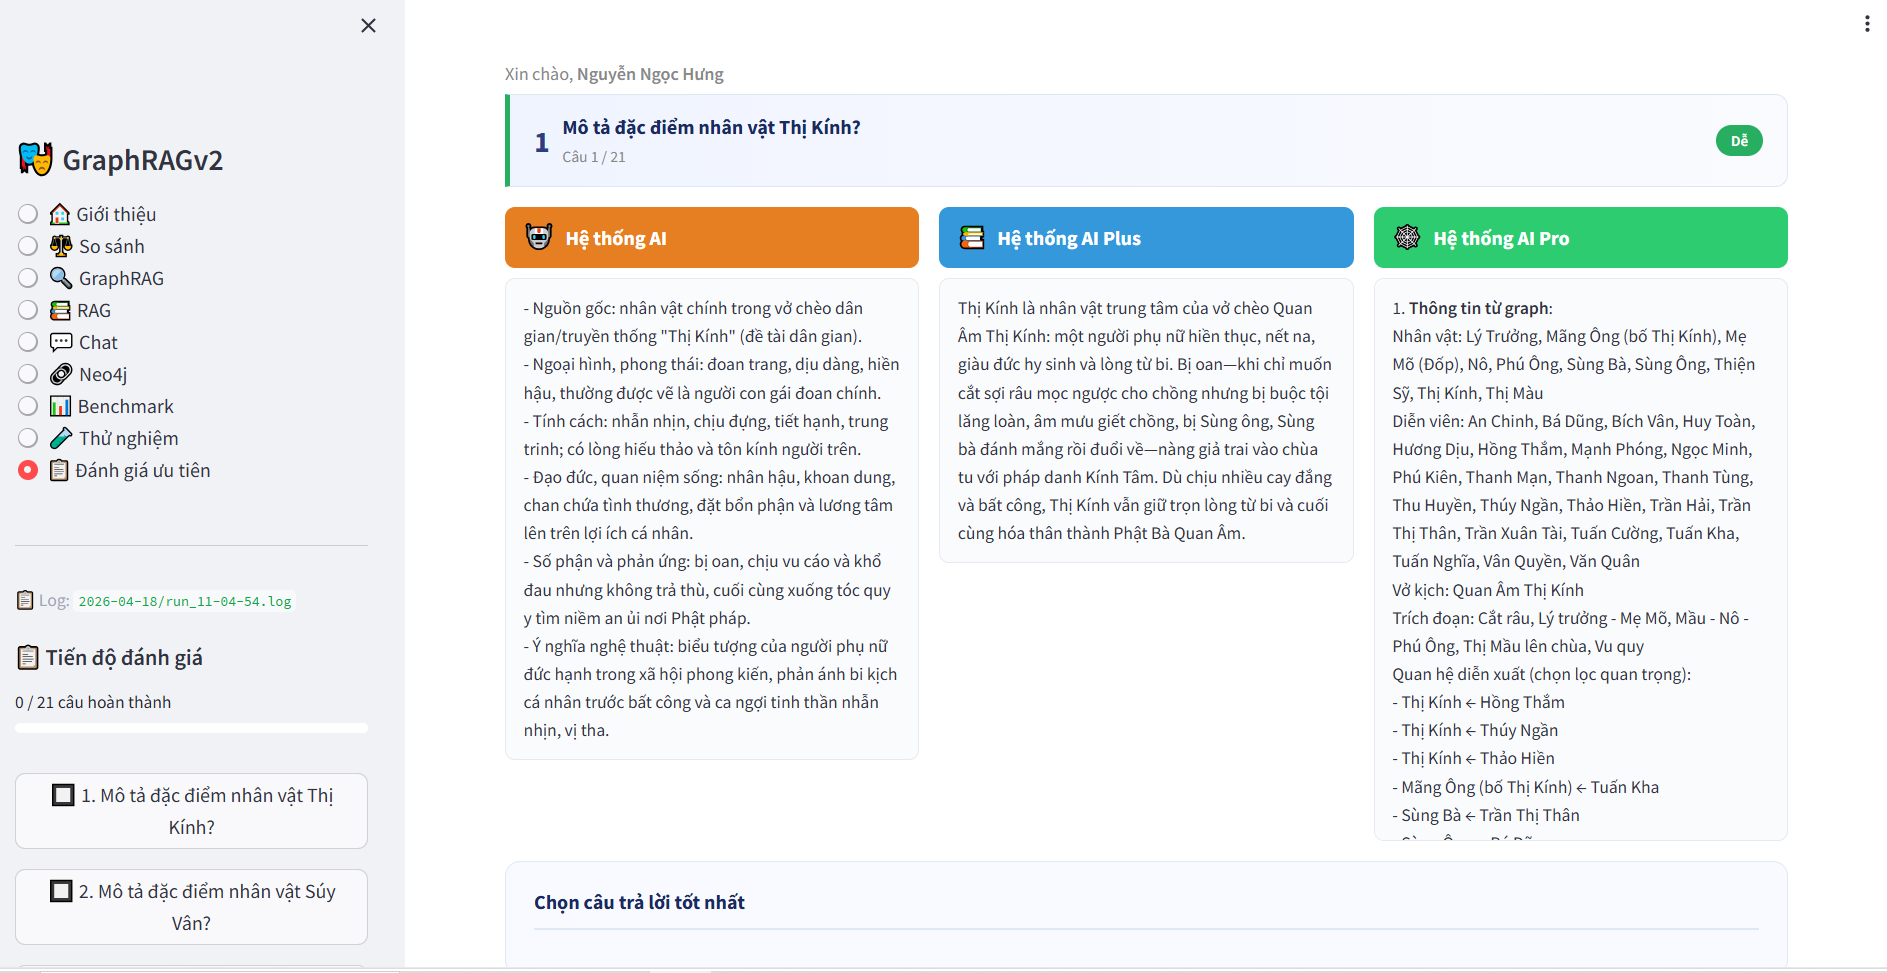
\includegraphics[width=0.9\linewidth]{figures//c4/preference.png}
    \caption{Giao diện thực nghiệm so sánh}
    \label{fig:preference}
\end{figure}

Khác với hình thức trước, Preference không yêu cầu chấm điểm theo thang nhiều mức mà chỉ yêu cầu phán xét tổng thể ``câu trả lời nào là hay nhất''. Định dạng so sánh ba cột trực tiếp giúp người tham gia dễ phát hiện các lỗi tinh tế như chi tiết sai lệch, thiếu sót về nhân vật hoặc mâu thuẫn nội dung --- những lỗi mà các độ đo tự động thường bỏ qua. Việc sử dụng câu trả lời sinh sẵn đảm bảo công bằng: mọi người tham gia đánh giá trên cùng một tập câu trả lời, loại trừ biến động giữa các lần gọi mô hình.

Đối tượng tham gia hình thức này là các chuyên gia có hiểu biết sâu về nghệ thuật Chèo. Kiến thức chuyên môn cho phép họ thẩm định các chi tiết đặc thù của miền --- như tính chính xác của tên nhân vật, mối quan hệ giữa vở diễn, hay sự tinh tế trong cách diễn đạt --- mà người dùng phổ thông khó nắm bắt. Đánh giá của chuyên gia do đó có độ tin cậy cao hơn khi so sánh trực tiếp chất lượng nội dung giữa các hệ thống.

\subsection{Kết quả kiểm nghiệm với người dùng}

\textit{Phần này tổng hợp kết quả của cả hai hình thức kiểm nghiệm. Do quá trình thu thập dữ liệu người dùng vẫn đang tiếp tục tại thời điểm viết báo cáo, các số liệu chi tiết sẽ được bổ sung trong phiên bản hoàn chỉnh.}

% [Placeholder — cập nhật khi có dữ liệu thu thập đầy đủ]
% - Kết quả hình thức 1 (sinh viên): phân bổ phiếu hệ thống tốt nhất, điểm trung bình ba tiêu chí theo từng hệ thống, phân tích theo phân nhóm hiểu biết Chèo.
% - Kết quả hình thức 2 (chuyên gia): phân bổ phiếu chọn, phân tích định tính từ ghi chú.
% - Đối sánh giữa đánh giá sinh viên và đánh giá chuyên gia.
% - Đối sánh giữa đánh giá chủ quan và đánh giá khách quan từ các độ đo ở Mục~\ref{sec:experiments}.

\subsection{Thảo luận trải nghiệm thực tế}

\textit{Phần thảo luận chi tiết sẽ được hoàn thiện khi có đầy đủ dữ liệu kiểm nghiệm người dùng. Dự kiến các điểm thảo luận bao gồm: sự tương đồng và khác biệt giữa đánh giá chủ quan và đánh giá khách quan bằng các độ đo tự động; khác biệt trong cách đánh giá giữa nhóm sinh viên và nhóm chuyên gia; các hạn chế còn lại của hệ thống được bộc lộ qua phản hồi thực tế; và ý nghĩa ứng dụng của hệ thống trong bảo tồn và truyền bá di sản nghệ thuật Chèo.}


